\section{Design of C-=-1}
\label{language-design}
%todo: mention novel, new, innovative
C-=-1 was designed as a compiled, low-level, non-garbage-collected programming language, similar to C, C++ or Rust.
What diffirentiates C-=-1 are its two founding principles: all code is executable at compile-time and support rich metaprogramming.
The primary purpose of the language was to investigate how these ideas influence software written in it \cite{grabski2022compilation}.

C-=-1 is a simple language, built with the minimum set of features needed to demonstrate the usefulness of the proposed metaprogramming features.
They are discussed further in chapter \ref{design:attributes_and_metaprogramming}.
The primary motivation for those mechanisms, is providing the programmer the ability to create domain specific static analysis and code generation tools, without creating a separate program.

\subsection{Type system}

C-=-1 type system borrows from C++.
Program may contain user defined classes, with members which may have limited accessibility.
Generic programming is achieved by the use of templates, although they are much more limited than the ones present in C++.
The user may also use pointers to objects, with arbitrary indirection (for example pointer to pointer to object).
Additionally, the language contains the concept of an \lstinline{interface}, similar to the one found in C\# \cite{hejlsberg2003c}.

\subsection{Attributes and metaprogramming}
\label{design:attributes_and_metaprogramming}

Metaprogramming in C-=-1 is based on attributes.
Attributes work in a manner similar to the ones found in C\#.
They are types, which may contain fields and methods.
They can also, be used to annotate other elements of the program, such as types, functions or variables.

In C-=-1 these attributes may implement special member functions that react to use of the annotated program element.
For example, an attribute that can be attached to a function, may implement \lstinline{onCall} special member function.
It will be called, at compile time, for each invocation of the annotated procedure.
Within the special method, the attribute will have access to the semantic model of the call site.
It may then modify the semantic model or report warnings or errors.


Listing \ref{lst:noDiscardCm1} contains an example of a C-=-1 attribute: \lstinline{noDiscard}.
It works in the same manner as the attribute of the same name present in C++17 \cite{ISO:cpp17}: if applied to a function, the result of that invoking procedure must be used.

To declare an attribute in C-=-1, the \lstinline{att} keyword is used.
After that, attribute targets should be listed in angled brackets, as in line 0 of Listing \ref{lst:noDiscardCm1}.
Attributes may target any number of language elements, including types, functions, variables and fields. %todo: switch target to smth else
Attribute from Listing \ref{lst:noDiscardCm1} declares two member functions: \lstinline{attach} in line 4 and \lstinline{onCall} in line 6.

\begin{minipage}{\linewidth}

	\begin{lstlisting}[
	  numbers=left,
	  firstnumber=0,
	  caption={noDiscard attribute in C-=-1},
	  aboveskip=0pt,
	  label={lst:noDiscardCm1}
	  ]
  public att<function> NoDiscard
  {
	public fn attach(f: functionDescriptor)
	{}
	public fn onCall(call: functionCallExpression*)
	{
	if(call._parentStatment != null<IInstruction>())
	  raiseError(
		&(call._pointerToSource),
		"Return value of a no-discard function is not used",
		123
	  );
	}
  }
  \end{lstlisting}
\end{minipage}

The \lstinline{attach} method is called after names of all of the program elements have been gathered, but before the compiler starts to analyze function bodies.
It is common accross all attribute targets and accepts the descriptor of the attached program element (function, field, type, etc.).
Only during call to \lstinline{attach} can the attribute change aspects of the program that affect function overload resolution, for example
whether a function is invokable at run or compile time.

The \lstinline{onCall} method is an example of a function reacting to usage of the annotated program element.
They are speciffic to a given attribute target.
Within this function, the attribute may analyze and modify the code, as well as raise errors or warnings.

Lines 6 to 11 of Listing \ref{lst:noDiscardCm1} are an example of a C-=-1 attribute providing static analysis.
The \lstinline{onCall} method checks whether the attached function is invoked in an expression or instruction context.
Calling a function as a statment means that the result of that invocation is discarded by the caller.
This is may indicate an error, when the function has no other side effects.
If that is the case, the attribute calls the \lstinline{raiseError} function, which is provided as a compiler intrinsic, that generates a compilation error.
The example presented in Listing \ref{lst:noDiscardCm1}, although very basic, demonstrates the ability to implement a form of static analysis that typically requires modyfining the compiler or creating an external tool.

\begin{minipage}{\linewidth}

	\begin{lstlisting}[
	  numbers=left,
	  firstnumber=0,
	  caption={Example of using noDiscard attribute from Listing \ref{lst:noDiscardCm1}},
	  aboveskip=0pt,
	  label={lst:noDiscardUsageCm1}
	  ]
  [noDiscard()]
  fn noDiscardFunction() -> usize;

  fn main() -> usize
  {
	noDiscardFunction();
	// error 123: Return value of
	// a no-discard function is not used
	let x = noDiscardFunction();     // ok
	let y = x + noDiscardFunction(); // ok
	return noDiscardFunction();      // ok
  }
  \end{lstlisting}
\end{minipage}

\section{Design of the compiler}
\label{compiler-design}

CTFEF apporach was created during implementation of the first compiler for the C-=-1 language\cite{grabski2022compilation}.
CTFEF compiler has four major components: Frontend, Interpreter, Compiler Interface and Backend.
Figure \ref{CTFE-first-compiler-structure} contains a diagram with an overview of how these parts interact with eachother, during the compilaton process.
Frontend, described in chapter \ref{frontend}, parses the code in the compiled language and constructs its intermediate representation, using interpreter's data structures.
It is used to analyze both user code and the Compiler Interface.
After the intermediate representation is constructed, it is passed to the Interpreter, which was described in chapter \ref{interpreter}.
Compiler Interface intermediate representation is then executed, using the user program as data.
This step converts the semantic model of the program into the backends intermediate language.
This process is further explained in chapter \ref{compiler-interface}.
Finaly the Backend generates the executable file.

\begin{figure}
	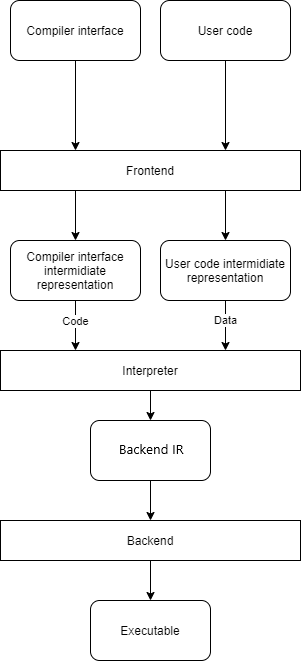
\includegraphics[height=14cm]{pictures/compiler-structure.png}
	\caption{CTFEF compiler structure}
	\label{CTFE-first-compiler-structure}
\end{figure}

\subsection{Frontend}
\label{frontend}

In the CTFEF approach, frontend serves the same role of constructing the programs intermediate representation, as in conventional compilers \cite{puntambekar:compiler_design}.
The major difference lays in the data structures used to describe the program.
For a CTFEF compiler to work, they must be accessible to the program running within the interpreter.
The increace of complexity, caused by using data structures accessible from interpreted code, depends on the design of the interpreter.


\subsection{Interpreter}
\label{interpreter}

In CTFEF, interpreter is main component of the compiler.
It executes the Compiler-Interface which translates the intermediate representation into the backend's assembly and serves as what is sometimes called the 'middle-end' of the compiler\cite{hsu2021llvm}.
To do it, it must be able to treat the program's intermediate representation both as code and data.

\begin{figure}
	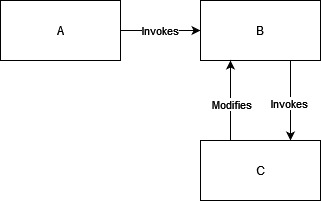
\includegraphics[width=7cm]{pictures/circular-function-reference.jpg}
	\caption{Example of circular reference in meta code}
	\label{circular-function-reference}
\end{figure}

An important consideration with implementing a CTFEF compiler, is what code can be executed at compile-time.
Depending on language design, it may be possible to introduce circular references between the functions that modify the codebase.
Figure \ref{circular-function-reference} contains a diagram of such a scenario.
\lstinline{A}, \lstinline{B} and \lstinline{C} are all functions.
If function \lstinline{B} is modified by function \lstinline{C} and \lstinline{C} invokes \lstinline{B}, the behaviour of function \lstinline{A} is unpredictable.
This problem will only be magnified by larger program sizes.


One of the possible solutions to the above mentioned problem is to limit which functions can be invoked at compiletime.
C-=-1 allows code within a compiletime context to invoke procedures only from other packages, declared explicitly as dependencies.
Circular references between packages, as in most other languages, are forbiden.
C-=-1 additionally prohibits modification of dependencies.
Therefore its is impossible for a function to modify a procedure it depends on.

\subsection{Compiler Interface}
\label{compiler-interface}

Compiler Interface translates the program's intermediate representation into the backend's assembly language.
This component is interpreted during compilation.
What is unique about CTFEF is that this part of the compiler can thus be written in the target language, during Stage 0 of the compiler bootstrapping process, as in the case of the C-=-1 compiler\cite{puntambekar:compiler_design, novillo2007gcc, grabski2022compilation}.

Compiler Interface is a regular code package that contains a function marked as the Compiler Interface Entry-point.
That procedure must accept a set of modules to be compiled and a Compilation Context that is used to generate the Backends assembly.
The module descriptors that are passed to the Compiler Interface are built by the frontend, as can be seen in figure \ref{CTFE-first-compiler-structure}.

After the Compiler Interface has finished generating backend assembly, the Compiler Backend is invoked to generate the binary executable.
\subsection{Backend}
\label{backend}

CTFEF does not put any additional requirements on compiler backend.
When using this pattern, an out-of-the-box backend library, can be used, as was the case with C-=-1 compiler.

The backend code must be invokable from within the interpreted program in the target language.
Depending on how the interpreter was designed, this may require significant effort. %todo: maybe other word
Compiler backends are large and for the Compiler Interface to take advantage of them, they must be fully available.
This means exposing each function and type within the library, to the interpreted code.
These bindings could feasibly be generated automatically \cite{marshalling_auto_generation}, but this technique was not used when implementing C-=-1 compiler.
